\section{Introduction}

This chapter provides a code-level breakdown of the six core algorithmic components of VidChain. Each section describes not just \textit{what} the code does but \textit{why} it was implemented that way, tracing design decisions back to the architectural constraints established in Chapter 4. All implementations are presented as structured pseudocode to communicate logic clearly without being tied to Python syntax.

% ─────────────────────────────────────────────
\section{Pipeline Execution: VideoChain.run()}
% ─────────────────────────────────────────────

\subsection{Overview}

The \texttt{VideoChain.run()} method is the central execution loop of the entire system. It is responsible for decoding the video frame by frame, constructing a shared context dictionary per frame, passing that context sequentially through every registered node, and accumulating the results into a unified temporal timeline.

\subsection{Algorithm}

\begin{algorithm}[H]
\caption{VideoChain.run(video\_path)}
\begin{algorithmic}[1]
\Require $video\_path$: path to a local video file
\Ensure $timeline$: list of fused event dictionaries

\State Extract audio track to temporary \texttt{.wav} file
\State Open video capture; read $fps$ and $total\_frames$
\State Initialise $timeline \gets [\,]$, $frame\_idx \gets 0$

\While{frames remain in video}
    \State Read next frame $F$
    \If{$frame\_idx \bmod frame\_skip \neq 0$}
        \State $frame\_idx \mathrel{+}= 1$; \textbf{continue}
    \EndIf

    \State $t \gets frame\_idx \;/\; fps$
    \State Initialise context $C \gets \{\text{video\_path}, \text{audio\_path}, \text{frame}: F, \text{time}: t\}$

    \State $skip \gets \texttt{False}$
    \For{each $node$ in $self.nodes$}
        \State $C \gets node.\text{process}(C)$
        \If{$C[\text{skip\_frame}] = \texttt{True}$}
            \State $skip \gets \texttt{True}$; \textbf{break}
        \EndIf
    \EndFor

    \If{$\neg\, skip$}
        \State Remove $C[\text{current\_frame}]$ \Comment{Free memory before storing}
        \State Append $C$ to $timeline$
    \EndIf

    \State $frame\_idx \mathrel{+}= 1$
\EndWhile

\State Close video capture
\State \Return $(timeline,\; audio\_path)$
\end{algorithmic}
\end{algorithm}

\subsection{Implementation Notes}

\textbf{Frame index vs.\ frame read.} The \texttt{frame\_skip} check is applied to $frame\_idx$ rather than skipping reads entirely. Every frame is read from the decoder, but only every $n$-th frame is processed. This is necessary because OpenCV's \texttt{cap.set(CAP\_PROP\_POS\_FRAMES)} seek is unreliable on certain codecs.

\textbf{Early abort on \texttt{skip\_frame}.} When the \texttt{AdaptiveKeyframeNode} sets \texttt{skip\_frame: True}, the loop breaks immediately without invoking any subsequent node. This achieves the 60--80\% compute saving reported in Chapter 3.

% ─────────────────────────────────────────────
\section{Adaptive Keyframe Filtering}
% ─────────────────────────────────────────────

\subsection{Overview}

The \texttt{AdaptiveKeyframeNode} acts as a computational firewall. Its purpose is to detect whether the current frame is visually distinct enough from the previous frame to justify running downstream heavy models.

\subsection{Algorithm}

\begin{figure}[H]
\centering
\begin{tikzpicture}[
    node distance=1.5cm,
    startstop/.style={draw, rectangle, rounded corners, minimum width=3cm, minimum height=1cm,text centered, fill=blue!15},
    process/.style={draw, rectangle, minimum width=3.5cm, minimum height=1cm, text centered, fill=orange!10},
    decision/.style={draw, diamond, aspect=2, minimum width=3.5cm, minimum height=1cm, text centered, fill=green!15},
    arrow/.style={thick,->,>=stealth}
]

\node (in) [startstop] {Input Frame};
\node (gray) [process, below=0.8cm of in] {Grayscale + Gaussian Blur};
\node (diff) [process, below=0.8cm of gray] {Compute AbsDiff(Ref, Curr)};
\node (dec) [decision, below=0.8cm of diff] {Change $> 8\%$?};
\node (skip) [startstop, left=2cm of dec, fill=red!15] {Skip Frame};
\node (upd) [process, below=0.8cm of dec] {Update Ref Frame};
\node (pass) [startstop, below=0.8cm of upd, fill=green!20] {Process Frame};

\draw [arrow] (in) -- (gray);
\draw [arrow] (gray) -- (diff);
\draw [arrow] (diff) -- (dec);
\draw [arrow] (dec) -- node[anchor=south] {No} (skip);
\draw [arrow] (dec) -- node[anchor=east] {Yes} (upd);
\draw [arrow] (upd) -- (pass);

\end{tikzpicture}
\caption{Visual Logic Flow: Adaptive Keyframe Filtering}
\label{fig:kf_flow}
\end{figure}

\begin{algorithm}[H]
\caption{AdaptiveKeyframeNode.process(context)}
\begin{algorithmic}[1]
\Require context $C$ containing \texttt{current\_frame} $F$
\Ensure $C[\text{skip\_frame}]$ set appropriately

\State $G \gets \text{GaussianBlur}(\text{Grayscale}(F),\; kernel=(21,21))$

\If{$prev\_gray = \texttt{None}$}
    \State $prev\_gray \gets G$
    \State $C[\text{skip\_frame}] \gets \texttt{False}$
    \State \Return $C$
\EndIf

\State $D \gets \text{AbsDiff}(prev\_gray,\; G)$
\State $nonzero \gets \text{CountNonZero}(D > diff\_cutoff)$
\State $change\_pct \gets (nonzero \;/\; |D|) \times 100$

\If{$change\_pct < change\_threshold$}
    \State $C[\text{skip\_frame}] \gets \texttt{True}$
\Else
    \State $prev\_gray \gets G$
    \State $C[\text{skip\_frame}] \gets \texttt{False}$
\EndIf

\State \Return $C$
\end{algorithmic}
\end{algorithm}

\subsection{Implementation Notes}

\textbf{Gaussian blur differencing.} A 21$\times$21 Gaussian blur removes high-frequency noise before the difference is computed, ensuring that the change percentage reflects genuine scene motion rather than sensor jitter.

\textbf{Reference update policy.} By only updating the reference when a genuine keyframe is accepted, the node measures change relative to the last \textit{meaningful} frame, preventing drift.

% ─────────────────────────────────────────────
\section{GraphRAG: Build and Query}
% ─────────────────────────────────────────────

\subsection{Build Algorithm}

\begin{algorithm}[H]
\caption{TemporalKnowledgeGraph.build\_from\_timeline(timeline)}
\begin{algorithmic}[1]
\Require $timeline$: list of fused event dictionaries
\Ensure Directed graph $G$ populated with temporal entity facts

\For{each event $e$ in $timeline$}
    \State $t \gets e[\text{time}]$
    \State Add timestamp node $t\_node \gets$ \texttt{"t:"}$t$ to $G$

    \For{each tracking string $s$ in $e[\text{tracking}]$}
        \State $entity \gets$ ExtractEntityID($s$)
        \If{$entity \neq \texttt{None}$}
            \State AddOrUpdateEntityNode($G$, $entity$, $t$)
            \State AddEdge($G$, $t\_node \to entity$, relation=\texttt{detects})
        \EndIf
    \EndFor

    \If{$|e[\text{objects}]| < 120$}
        \For{each YOLO object $obj$ in ParseYOLO($e[\text{objects}]$)}
            \State AddOrUpdateEntityNode($G$, $obj$, $t$)
        \EndFor
    \EndIf

    \If{$e[\text{ocr}] \neq \texttt{None}$}
        \State AddOCRNode($G$, $e[\text{ocr}]$, $t$)
        \State AddEdge($G$, $t\_node \to ocr\_node$, relation=\texttt{screen\_shows})
    \EndIf

\EndFor
\end{algorithmic}
\end{algorithm}

\subsection{Implementation Notes}

\textbf{The 120-character guard.} This threshold distinguishes between short structured YOLO output and free-form VLM prose, ensuring only structured entities are indexed.

% ─────────────────────────────────────────────
\section{Recursive Map-Reduce Summarisation}
% ─────────────────────────────────────────────

\begin{figure}[H]
\centering
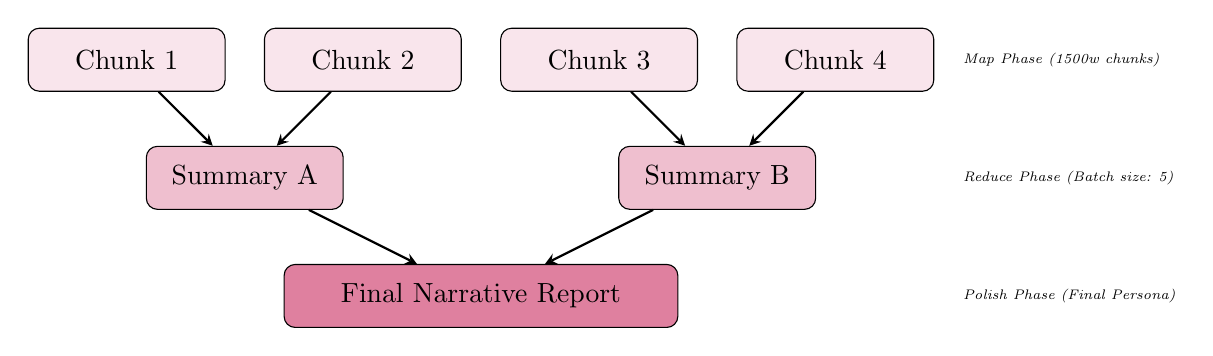
\begin{tikzpicture}[
    level/.style={draw, rectangle, rounded corners, minimum width=2.5cm, minimum height=0.8cm, text centered, fill=purple!10},
    arrow/.style={thick,->,>=stealth}
]

% Level 0
\node[level] (L0_1) at (0,0) {Chunk 1};
\node[level] (L0_2) at (3,0) {Chunk 2};
\node[level] (L0_3) at (6,0) {Chunk 3};
\node[level] (L0_4) at (9,0) {Chunk 4};

% Level 1
\node[level, fill=purple!25] (L1_1) at (1.5, -1.5) {Summary A};
\node[level, fill=purple!25] (L1_2) at (7.5, -1.5) {Summary B};

% Level 2
\node[level, fill=purple!50, minimum width=5cm] (L2) at (4.5, -3) {Final Narrative Report};

% Arrows
\draw [arrow] (L0_1) -- (L1_1);
\draw [arrow] (L0_2) -- (L1_1);
\draw [arrow] (L0_3) -- (L1_2);
\draw [arrow] (L0_4) -- (L1_2);
\draw [arrow] (L1_1) -- (L2);
\draw [arrow] (L1_2) -- (L2);

\node[anchor=west, font=\tiny\itshape] at (10.5, 0) {Map Phase (1500w chunks)};
\node[anchor=west, font=\tiny\itshape] at (10.5, -1.5) {Reduce Phase (Batch size: 5)};
\node[anchor=west, font=\tiny\itshape] at (10.5, -3) {Polish Phase (Final Persona)};

\end{tikzpicture}
\caption{Recursive Map-Reduce Hierarchical Collapse Structure}
\label{fig:mapreduce_viz}
\end{figure}

\begin{algorithm}[H]
\caption{Recursive Narrative Map-Reduce}
\begin{algorithmic}[1]
\Procedure{GenerateSummary}{$\mathcal{T}, mode$}
    \State $chunks \gets \text{ChunkByWordLimit}(\mathcal{T}, 1500)$
    \State $chapter\_summaries \gets$ MapPhase($chunks$)
    \State \textbf{return} \Call{RecursiveReduce}{$chapter\_summaries, mode$}
\EndProcedure

\Statex
\Procedure{RecursiveReduce}{$\mathcal{S}_{list}, mode$}
    \If{$\text{length}(\mathcal{S}_{list}) = 1$}
        \State \textbf{return} FinalPolish($\mathcal{S}_{list}[0], mode$)
    \EndIf
    \State $\mathcal{G} \gets \text{Group}(\mathcal{S}_{list}, batch\_size=5)$
    \State $\mathcal{R} \gets [ ]$
    \For{each batch $g \in \mathcal{G}$}
        \State $r \gets \text{LLM}(\text{Prompt}_{reduce}, g)$
        \State $\mathcal{R}.\text{append}(r)$
    \EndFor
    \State \textbf{return} \Call{RecursiveReduce}{$\mathcal{R}, mode$}
\EndProcedure
\end{algorithmic}
\end{algorithm}

% ─────────────────────────────────────────────
\section{RAG Engine and Session Management}
% ─────────────────────────────────────────────

\subsection{Session Lifecycle Algorithm}

\begin{algorithm}[H]
\caption{Session Lifecycle: Create, Ingest, Query, Delete}
\begin{algorithmic}[1]

\Statex \textbf{INGEST}
\State Lock $session[\text{video\_id}] \gets video\_id$ immediately
\State Lock $session[\text{video\_path}] \gets video\_source$
\State Save session to disk
\State Dispatch \texttt{\_background\_ingest()} as background task

\Statex \textbf{DELETE}
\State $video\_id \gets session[\text{video\_id}]$
\State \texttt{ChromaDB.delete(where=\{video\_id\})}
\State Delete \texttt{knowledge\_graphs/graph\_\{video\_id\}.pkl}
\State Delete \texttt{knowledge\_bases/\{video\_id\}.json}
\State Delete \texttt{sessions/\{session\_id\}.json}
\end{algorithmic}
\end{algorithm}

\subsection{Final Implementation Notes}

\textbf{Thermal Mitigation.} The implementation includes a $10\,\text{ms}$ sleep interval in the processing loop to provide the RTX 3050 with "thermal breathing room," preventing clock-speed throttling.

\textbf{VRAM-Aware Lazy Loading.} Node initialization is staggered by 2 seconds to ensure the CUDA context is stable before the next model claims its VRAM allocation.

\textbf{Memory Isolation.} Every session deletion triggers a "Three-artefact purge" to guarantee that no residual data influences future queries.

% ─────────────────────────────────────────────
\section{Summary}
% ─────────────────────────────────────────────

This chapter has presented the implementation of all six core algorithmic components of VidChain. Each was examined at the level of its controlling algorithm and then analysed for the non-obvious implementation decisions that distinguish it from a naive approach. The \texttt{VideoChain.run()} loop's sequential read strategy, the keyframe node's reference-frame update policy, the graph builder's VLM-prose guard, the summariser's word-budget chunking, the retrieval pipeline's post-rerank chronological re-sort, and the session manager's three-artefact purge --- each of these represents a deliberate engineering choice made in response to a concrete failure mode encountered during development. Chapter 6 presents the empirical results that validate these decisions.